\subsection{Variations on the EOQ model}
\label{sec:variations-eoq-model}

\begin{question}
  When choosing an inventory policy, i.e., a policy that decides when
  and how much to order, we need to understand the environment first
  in which the policy is going to operate. Can you use
  Question~\ref{ex:1} to come up with a characterization of the environment? 
  \begin{solution}
    A simple starting point is provided by this table.
    \begin{table}[h]
      \centering
    \begin{tabular}{l|l|l|l}
      Environment && &  \\ \hline
Demand & variability &deterministic/constant & Stochastic \\ 
& substitution effects & yes & no \\
\hline Supply & Lead time & $L=0$& $L>0$ \\ 
& perishable items & yes & no\\
& Joint ordering & yes & no\\
& Order size constraints &yes & no \\
\hline Cost structure &Ordering cost & $A=0$ & $A>0$ \\ 
& holding cost & $h=0$ &$h>0$ \\
& fixed backlog cost & $\pi=0$ &$\pi>0$\\
&variable backlog cost & $b=0$ &$b>0$\\
&lost sales cost &$k=0$ & $k>0$ \\
&quantity discounts &yes & no \\
\hline KPIs &fill rate $S$ & yes & no\\ 
& cycle service level &yes& no\\
    \end{tabular}
    \caption{(Incomplete) characterization of the environment of inventory policies}
      \label{tab:environment}
    \end{table}
  \end{solution}
\end{question}

\begin{question}
  Characterize the EOQ model by means of the table of the previous
  question.
  \begin{solution}
    \begin{table}[h]
      \centering
    \begin{tabular}{l|l|l|l}
      Environment && &  \\ \hline
Demand & variability &\boxed{deterministic/constant} & Stochastic \\ 
& substitution effects & yes & \boxed{no} \\
\hline Supply & Lead time & \boxed{$L=0$}& $L>0$ \\ 
& perishable items & yes & \boxed{no}\\
& Joint ordering & yes & \boxed{no}\\
& Order size constraints &yes & \boxed{no} \\
\hline Cost structure &Ordering cost & $A=0$ & $\boxed{A>0}$ \\ 
& holding cost & $h=0$ & $\boxed{h>0}$ \\
& fixed backlog cost & $\pi=0$ & $\boxed{\pi=\infty}$\\
&variable backlog cost & $b=0$ &$\boxed{b=\infty}$\\
&lost sales cost &$k=0$ & $\boxed{k=\infty}$ \\
&quantity discounts &yes & \boxed{no} \\
\hline KPIs &fill rate & $\boxed{S=1}$ & no\\ 
& cycle service level &yes& no\\
    \end{tabular}
    \caption{EOQ model }
      \label{tab:environment}
    \end{table}
  \end{solution}
\end{question}

\begin{question}
  In the next set of questions we are going to modify the assumptions
  of the EOQ model with the aim to investigate how the environment
  affects the inventory policy. For the sake of comparison, sketch how the inventory behaves over time for the EOQ model and write down the cost function.

  \begin{solution}
\begin{center}
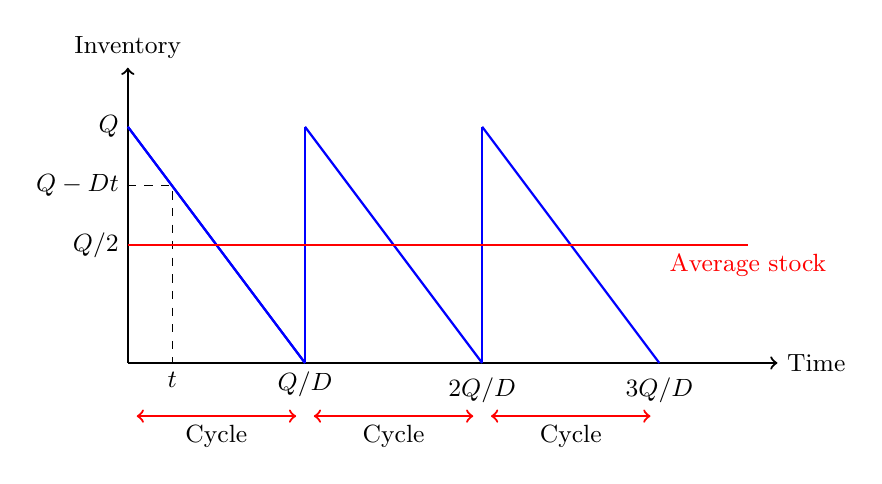
\begin{tikzpicture}[x=0.75cm,y=0.015cm]
\small
\draw[thick,->] (0,0) -- (11,0) node[right] {Time};
\draw[thick,->] (0,0) -- (0,250) node[above] {Inventory};
\draw[] (0,200) node[left] {$Q$};
\draw[color=blue,thick] (0,200) -- (3,0);
\draw[] (0.75,0) node[below] {$t$};
\draw[] (0,150) node[left] {$Q-Dt$};
\draw[dashed] (0,150) -- (0.75,150) -- (0.75,0);
\draw[] (3,0) node[below] {$Q / D$};
\foreach \y in {1,...,3}{
	\draw[color=blue,thick] (3*\y-3,200) -- (3*\y,0);}
\foreach \y in {1,2}{
	\draw[color=blue,thick] (3*\y,0) -- (3*\y,200);}
\foreach \y in {2,3}{
	\draw[] (3*\y,-5) node[below] {\y $Q/D$};}
\draw[] (0,100) node[left] {$Q / 2$};
\draw[color=red,thick] (0,100) -- (10.5,100) node[below] {Average stock};
\foreach \y in {0,...,2}{
	\draw[color=red,thick,<->] (3*\y+0.15,-45) -- (3*\y+3-0.15,-45);
	\draw[] (3*\y+1.5,-45) node[below] {Cycle};}
\end{tikzpicture}
\end{center}

The total cost for one cycle is the order cost plus the inventory cost. The order cost is $A$, the inventory cost is the total area of the triangle times $h$, i.e. 
\begin{equation*}
  \frac h2\text{height}\cdot\text{base} = \frac h 2 Q\cdot \frac QD= \frac h2 \frac{Q^2}D.
\end{equation*}
The average cost per unit time is this total cost divided by the duration of one cycle, which is $Q/D$. Therefore, the average cost is
\begin{equation*}
\frac A{Q/D}+  \frac{ h/2 \cdot Q^2/D}{Q/D} = \frac h 2 \frac {Q^2} D\cdot \frac D/Q = \frac D Q A + \frac h2 Q.
\end{equation*}

\begin{center}
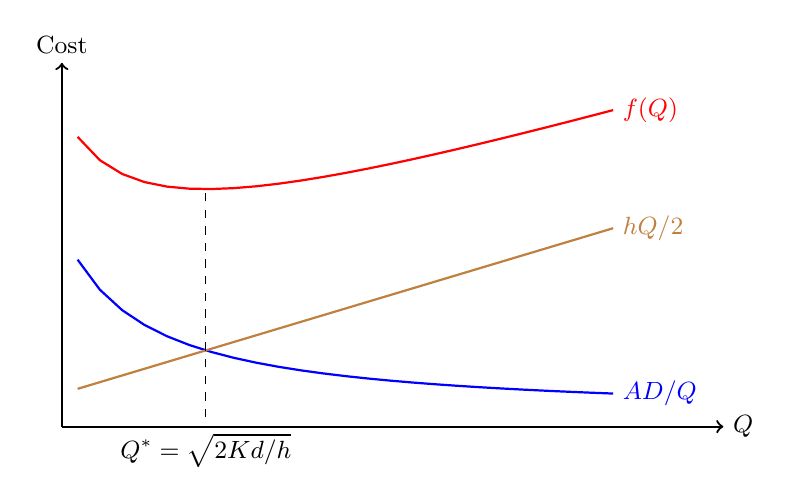
\begin{tikzpicture}[x=0.02cm,y=0.06cm]
\small
\def\c{1} 
\def\K{100} 
\def\h{0.2} 
\def\d{20} 
\pgfmathsetmacro{\Q}{sqrt(2)*sqrt(\K)*sqrt(\d)/sqrt(\h)}
\pgfmathsetmacro{\f}{sqrt(2)*sqrt(\K)*sqrt(\d)*sqrt(\h)+\c*\d}	
\draw[thick,->] (50,-2) -- (470,-2) node[right] {$Q$};
\draw[thick,->] (50,-2) -- (50,75) node[above] {Cost};
\draw[color=blue,thick,domain=60:400] plot (\x,{\d*\K/\x}) node[right] {$AD / Q$};
\draw[color=brown,thick,domain=60:400] plot (\x,{\h*\x/2}) node[right] {$hQ / 2$};
\draw[color=red,thick,domain=60:400] plot (\x,{\d*\K/\x+\c*\d+\h*\x/2}) node[right] {$f(Q)$};
\draw (\Q,-1.5) node[below] {$Q^{*} = \sqrt{2Kd / h}$};
\draw[dashed] (\Q,0) -- (\Q,\f);
\end{tikzpicture}
\end{center}

  \end{solution}
\end{question}

\begin{question}
  It is very important to memorize that the total inventory cost for
  the EOQ model is quite insensitive to the actual order quantity
  $Q$. Show this for the case with $A=100$, $h=0.2$, and $D=20$. What
  happens to the total cost if $Q=60, 80, \ldots 200$?
  \begin{solution}
From the EOQ formula
\begin{itemize}
\item $Q^{*} \approx 141.42$ units
\item $f(Q^{*}) \approx \mathdollar 48.28$
\end{itemize}

\begin{center}
\footnotesize
\begin{tabular}{rrrrr}
\toprule
$Q$     & $AD/Q$  &  $hQ/2$  & $f(Q)$ \\
\midrule
    60    & 33.33 &  6.00  & 59.33 \\
    80    & 25.00 &  8.00  & 53.00 \\
    100   & 20.00 &  10.00 & 50.00 \\
    120   & 16.67 &  12.00 & 48.67 \\
    140   & 14.29 &  14.00 & 48.29 \\
    160   & 12.50 &  16.00 & 48.50 \\
    180   & 11.11 &  18.00 & 49.11 \\
    200   & 10.00 &  20.00 & 50.00 \\
\bottomrule
\end{tabular}
\end{center}
  \end{solution}
\end{question}

\begin{question}
  As a first variation, what would you change/do if the lead time $L$
  is no longer 0, but becomes positive? (Thus, all the other
  assumptions of the EOQ model stay the same, only the lead time
  becomes positive.)  In other words, how would you change the EOQ
  policy, and determine when and how to order?
  \begin{solution}
    Since the backlog costs are infinite, backlogging is not
    desirable, hence we order early. See the graph: 
\begin{center}
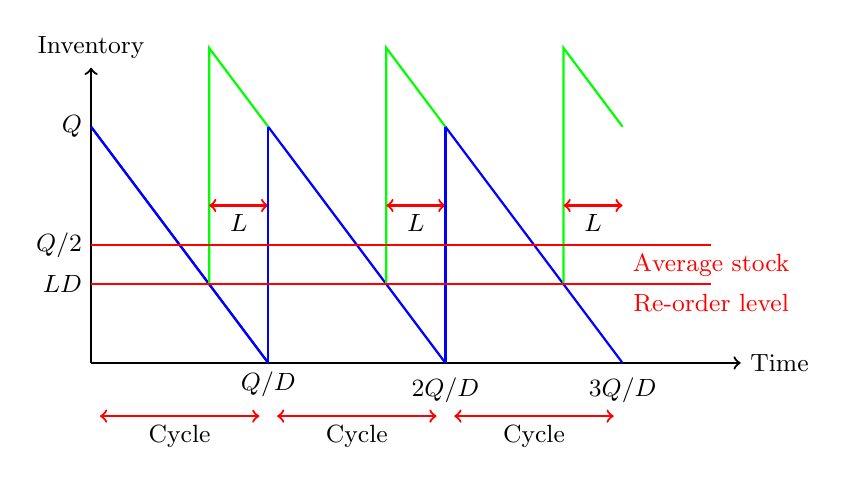
\begin{tikzpicture}[x=0.75cm,y=0.015cm]
\small
\draw[thick,->] (0,0) -- (11,0) node[right] {Time};
\draw[thick,->] (0,0) -- (0,250) node[above] {Inventory};
\draw[] (0,200) -- (0,200) node[left] {$Q$};
\draw[color=blue,thick] (0,200) -- (3,0);
\draw[] (3,0) node[below] {$Q / D$};
\foreach \y in {1,...,3}{
	\draw[color=blue,thick] (3*\y-3,200) -- (3*\y,0);
	\draw[color=green,thick] (3*\y-3+2,200/3) -- (3*\y-3+2,200/3*4) -- (3*\y,200);
	\draw[color=red,thick,<->] (3*\y-3+2,200/3*2) -- (3*\y,200/3*2);
	\draw[] (3*\y-3+2.5,200/3*2) node[below] {$L$};}
\foreach \y in {1,2}{
	\draw[color=blue,thick] (3*\y,0) -- (3*\y,200);}
\foreach \y in {2,3}{
	\draw[] (3*\y,-5) node[below] {\y $Q/D$};}
\draw[] (0,100) node[left] {$Q / 2$};
\draw[color=red,thick] (0,100) -- (10.5,100) node[below] {Average stock};
\draw[] (0,200/3) node[left] {$L D$};
\draw[color=red,thick] (0,200/3) -- (10.5,200/3) node[below] {Re-order level};
\foreach \y in {0,...,2}{
	\draw[color=red,thick,<->] (3*\y+0.15,-45) -- (3*\y+3-0.15,-45);
	\draw[] (3*\y+1.5,-45) -- (3*\y+1.5,-45) node[below] {Cycle};}
\end{tikzpicture}
\end{center}
    
This new policy can be described in a simple way by introducing the
concept of \emph{inventory position}, that is, all stock on-hand plus
the replenishments under way. The green graph above illustrates the
inventory position $IP$. When $IP$ hits the lead time demand $L D$,
i.e., the lead time $L$ times the demand $D$, we should order
$Q$. During the lead time $L$ the demand will be met from on-hand
stock. When the replenishment arrives a lead time $L$ later, it
arrives just in time to meet the demand again .
  \end{solution}
\end{question}

\begin{question}

How can we decompose leadtime?

\begin{solution}
TBD
\end{solution}

\end{question}



\begin{question}
  What would happen if it is allowed to backorder demand, in other
  words $b>0$, but $\pi = 0$? (We set $L=0$ again.)
  \begin{solution}
\begin{center}
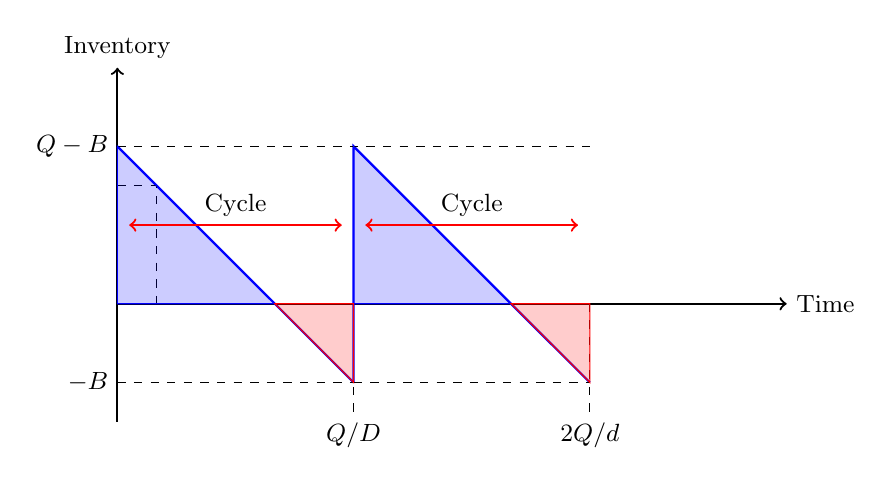
\begin{tikzpicture}[x=1cm,y=0.01cm]
\small

\draw[thick,->] (0,0) -- (8.5,0) node[right] {Time};
\draw[thick,->] (0,-150) -- (0,300) node[above] {Inventory};

\draw[] (0,200) node[left] {$Q - B$};

\draw[color=blue,thick] (0,200) -- (3,-100);

\draw[] (0,-100) node[left] {$-B$};
\draw[dashed] (0,-100) -- (3,-100);

%\draw[] (0,150) node[left] {$Q - B - Dt$};
%\draw[] (0.5,0) node[below] {$t$};
\draw[dashed] (0,150) -- (0.5,150) -- (0.5,0);

%\draw[] (2,0) node[below] {$(Q - B) / d$};

\draw[dashed] (3,0) -- (3,-140) node[below] {$Q / D$};

\draw[color=blue,thick] (3,-100) -- (3,200) -- (6,-100);
%\draw[] (5,0) node[below] {$(2Q - B) / d$};
\draw[dashed] (6,0) -- (6,-140) node[below] {$2Q / d$};
\draw[dashed] (0,200) -- (6,200);
\draw[dashed] (3,-100) -- (6,-100);

\draw [draw=blue,fill=blue,fill opacity=0.2] (0,0) -- (0,200) -- (2,0) -- cycle;
\draw [draw=blue,fill=blue,fill opacity=0.2] (3,0) -- (3,200) -- (5,0) -- cycle;
\draw [draw=red,fill=red,fill opacity=0.2] (2,0) -- (3,-100) -- (3,0) -- cycle;
\draw [draw=red,fill=red,fill opacity=0.2] (5,0) -- (6,-100) -- (6,0) -- cycle;

\foreach \y in {0,1}{
	\draw[color=red,thick,<->] (3*\y+0.15,100) -- (3*\y+3-0.15,100);
	\draw[] (3*\y+1.5,100) node[above] {Cycle};}
\end{tikzpicture}
\end{center}

The blue area is
\begin{equation*}
\frac12  \text{height}\cdot\text{base} = \frac12 (Q-B)\frac{(Q-B)}{D}=\frac{(Q-B)^2}{2D}
\end{equation*}
while the red area is
\begin{equation*}
  \frac12 B \frac{B}{D}=\frac{B^2}{2D}.
\end{equation*}
Thus, the time average cost is the total cost divided by the cycle lenght $Q/D$:
\begin{equation*}
  \begin{split}
  F(Q) 
&= \frac{D}{Q}A + \frac{h(Q-B)^2/2D}{Q/D} + \frac{b B^2/2D}{Q/D} \\
&= \frac{D}{Q}A + h\frac{(Q-B)^2}{2Q} + b \frac{B^2}{2Q}.
  \end{split}
\end{equation*}
Check that by setting $B=0$ you get the old EOQ result.
\end{solution}
\end{question}

\begin{question}
  What happens to the optimal cost if you allow for backorders?  What
  will happen to the optimal order quantity $Q$, will it become larger or smaller? 
  \begin{solution}
    The cost must become lower, since we remove a constraint. 

    Let's see by how much.  This is not so simple, however, because we
    now have two `controls' (or degrees of freedom): the order
    quantity $Q$ and the backorder level $B$. Even though it is
    possible to find a closed form solution for the optimal values of
    $Q$ and $B$, here we satisfy ourselves with a graphical analysis.
    We are going to make a plot of the total cost as a function of $Q$
    for various values of $B$.

    Here is an example. Take $A=100$, $h=0.2$, $D=20$, $B=10$, $b=1$.

\begin{center}
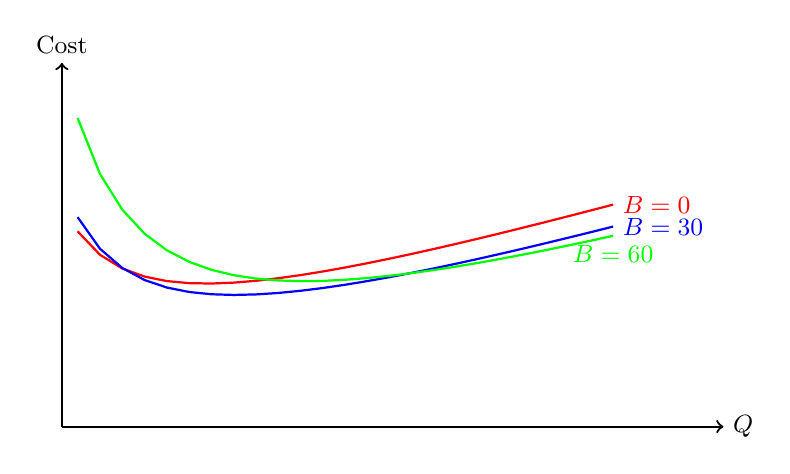
\begin{tikzpicture}[x=0.02cm,y=0.06cm,
declare function = {
f(\Q) = \D*\A/\Q+\h/2*(\Q-\B)/\Q*(\Q-\B)+\b/2*\B/\Q*\B; }
]
\small
\def\A{100} 
\def\h{0.2} 
\def\D{20} 
\def\b{1}
%\def\B{0}
%\pgfmathsetmacro{\f}{sqrt(2)*sqrt(\A)*sqrt(\D)*sqrt(\h)}	
\draw[thick,->] (50,-2) -- (470,-2) node[right] {$Q$};
\draw[thick,->] (50,-2) -- (50,75) node[above] {Cost};
%\draw[color=red,thick,domain=60:400] plot function{\D*\A/x+\h*x/2} node[right] {$B=0$};
%\draw[color=red,thick,domain=60:400] plot (\x,{\D*\A/\x+1*pow(\x,2)}) node[right] {$B=0$};
\def\B{0}
\draw[color=red,thick,domain=60:400] plot (\x,{f(\x)}) node[right] {$B=\B$};
\def\B{30}
\draw[color=blue,thick,domain=60:400] plot (\x,{f(\x)}) node[right] {$B=\B$};
\def\B{60}
\draw[color=green,thick,domain=60:400] plot (\x,{f(\x)}) node[below] {$B=\B$};
% \begin{axis}
% \addplot {f(x)};
% \end{axis}
\end{tikzpicture}
\end{center}


We see that the curve related to $B=30$, i.e., the
blue curve, achieves the lowest point of each of the three graphs.
The minimum of the blue curve is realized a bit to the right of the
minimum of the $B=0$ curve, i.e., the red curve.  Thus, from the
graphs, by setting $B=30$ and $Q$ a bit larger than the optimal value
for the EOQ model, we can lower the cost a bit.

% \begin{tikzpicture}[domain=-1:1,yscale=2,xscale=4,smooth]
% %\fill[gray] (-1.2,-1.2) rectangle (1.2,2.5);
% \draw[very thin] (-1.1,-1.1) grid[step=.5] (1.1,2.4);
% \draw[thick,->] (-1.2,0) -- (1.2,0);
% \draw[thick,->] (0,-1.2) -- (0,2.5);
% \draw[color=red] plot[id=1] function{cos(pi*x)};
% \draw[color=blue,thick] plot[id=2] function{cos(pi*x)+cos(2*pi*x)/2};
% \draw[color=green!50!black,thick] plot[id=3] function{cos(pi*x) + cos(2*pi*x)/2 + cos(3*pi*x)/3};
% \draw[color=yellow,thick] plot[id=4] function{cos(pi*x) + cos(2*pi*x)/2 + cos(3*pi*x)/3 + cos(4*pi*x)/4};
% %\draw<5->[color=cyan,thick] plot[id=5] function{cos(pi*x) + cos(2*pi*x)/2 + cos(3*pi*x)/3 + cos(4*pi*x)/4 + cos(5*pi*x)/5};
% \end{tikzpicture}

% \begin{tikzpicture}[
% declare function={ Nprime(\x)                 = 1/(sqrt(2*pi))*exp(-0.5*(pow(\x,2))); 
%                    d2(\x,\y,\KK,\RR,\SIG)     = (ln(\x/\KK)+(\RR-(pow(\SIG,2)/2)*\y))/(\SIG*(sqrt(\y)));
%                    myfun(\x,\y,\KK,\RR,\SIG)  = exp(-\RR*\y)*Nprime(d2(\x,\y,\KK,\RR,\SIG))/(\x*\SIG*sqrt(\y));
%                  },
% ]
% \begin{axis}[y domain=0.01:0.3,domain=95:105,view={150}{20}]
% \addplot3[surf] {myfun(x,y,100,0,0.09)};
% \end{axis}
% \end{tikzpicture}

  \end{solution}
\end{question}

\begin{question}
  What would you do if $b=0$, $\pi > 0$ and $h>0$? 
  \begin{solution}

TBD. 
    We have two alternatives. If we decide to keep no inventory, we
    only have to pay for backlogging demand. 

    Demand needs to enter in discrete amounts, for otherwise paying
    $\pi$ per demand becomes a bit strange.
  \end{solution}
\end{question}

\begin{question}We can also decide to reject demand rather than
  backlog it. Can you sketch the consequences on the behavior of the
  inventory level?  What happens to the order quantity $Q$?  What are
  the consequences in terms of cost, does it become lower or higher?
  \begin{solution}
    The influence on the cost is qualitatively easy. Once again we
    relax a constraint, hence it must be possible to reduce the
    average cost. Again, we are trying to find out by how much. 

    \begin{remark}
      I added this remark as a postscript to the analysis below. The
      solution here is quite messy because, while solving it, I made a
      few mistakes and conceptual errors. Despite this, I decided to
      keep the mistakes in with the aim to show you what went wrong,
      how I saw that things were wrong, and my attempts to repair
      it. The take-away message is that you see that making mistakes
      is part of the learning process\ldots for all of us\ldots
    \end{remark}

    Let's assume we order every $T$ periods.

\begin{center}
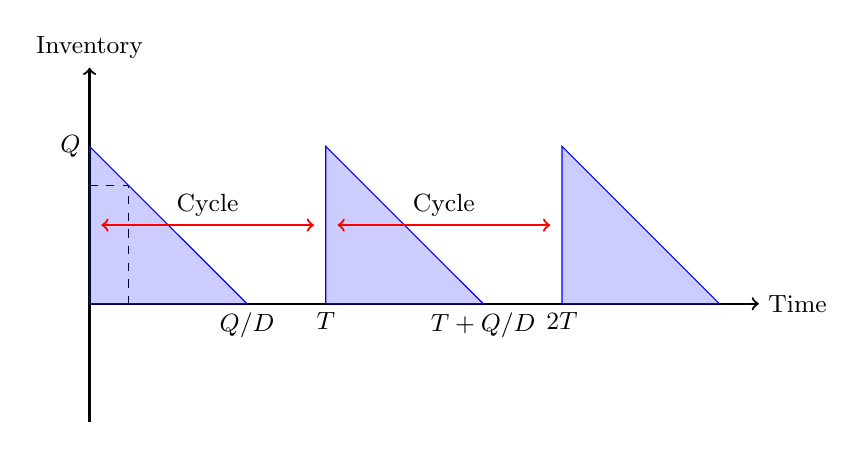
\begin{tikzpicture}[x=1cm,y=0.01cm]
\small

\draw[thick,->] (0,0) -- (8.5,0) node[right] {Time};
\draw[thick,->] (0,-150) -- (0,300) node[above] {Inventory};

\draw[] (0,200) node[left] {$Q$};

%\draw[color=blue,thick] (0,200) -- (3,-100);


%\draw[] (0,150) node[left] {$Q - B - Dt$};
%\draw[] (0.5,0) node[below] {$t$};
\draw[dashed] (0,150) -- (0.5,150) -- (0.5,0);

%\draw[] (2,0) node[below] {$(Q - B) / d$};

\draw[] (2,0) node[below] {$Q/D$};
\draw[] (3,0) node[below] {$T$};

%\draw[color=blue,thick] (3,-100) -- (3,200) -- (6,-100);
%\draw[] (5,0) node[below] {$(2Q - B) / d$};
\draw[] (5,0) node[below] {$T+Q/D$};
\draw[] (6,0) node[below] {$2T$};
%\draw[dashed] (0,200) -- (6,200);
%\draw[dashed] (3,-100) -- (6,-100);

\draw [draw=blue,fill=blue,fill opacity=0.2] (0,0) -- (0,200) -- (2,0) -- cycle;
\draw [draw=blue,fill=blue,fill opacity=0.2] (3,0) -- (3,200) -- (5,0) -- cycle;
\draw [draw=blue,fill=blue,fill opacity=0.2] (6,0) -- (6,200) -- (8,0) -- cycle;

\foreach \y in {0,1}{
	\draw[color=red,thick,<->] (3*\y+0.15,100) -- (3*\y+3-0.15,100);
	\draw[] (3*\y+1.5,100) node[above] {Cycle};}
\end{tikzpicture}
\end{center}

The average cost is the ordering cost plus the inventory cost plus the
cost of lost demand. We already analyzed the cost of the first two
terms. The loss cost is related to all demand lost between the time
$Q/D$ (i.e., the timer it takes the demand to consume $Q$) and the
next order moment $T$. The lost demand is
$DT-Q$. Thus, the average cost becomes
\begin{equation*}
  \begin{split}
  f(Q) 
&= \frac A T + \frac h2 \frac{Q\cdot Q/D}{T}+k \frac{DT-Q}T \\
&= \frac A T + \frac{hQ^2}{2DT}+k (D-\frac QT). 
  \end{split}
\end{equation*}

Take $A=100$, $h=0.2$, $D=20$, $k=1$. As a first attempt, take $T=D/Q^*$ (for the EOQ quantity $Q^*$.) Since $Q^* \approx 141$ and $D=200$, we take $T=200/141\approx 1.4$. \marginpar{This is were I made my first mistake, I copied the wrong numbers.}

\begin{center}
\begin{tikzpicture}[x=0.02cm,y=0.06cm,
declare function = {
f(\Q) = \A/\T+\h/2*\Q/\D*\Q/\T+\k*(\D*\T-\Q); }
]
\small
\def\A{100} 
\def\h{0.2} 
\def\D{20} 
\def\k{1}
%\pgfmathsetmacro{\f}{sqrt(2)*sqrt(\A)*sqrt(\D)*sqrt(\h)}	
\draw[thick,->] (50,-2) -- (470,-2) node[right] {$Q$};
\draw[thick,->] (50,-2) -- (50,75) node[above] {Cost};
\def\T{1.2}
\draw[color=blue,thick,domain=60:400] plot (\x,{f(\x)}) node[right] {$T=\T$};
\def\T{1.5}
\draw[color=red,thick,domain=60:400] plot (\x,{f(\x)}) node[right] {$T=\T$};
\def\T{2.0}
\draw[color=red,thick,domain=60:400] plot (\x,{f(\x)}) node[right] {$T=\T$};
\end{tikzpicture}
\end{center}

Now I wonder why the graph for $T=2$ becomes negative. I guess I did
something wrong, but what?  First I'm checked the cost function. The
only component that can give negative values is
$k(DT-Q)$. \marginpar{As it turned out, I also copied the formula
  incorrectly.} So, when the cost is negative,
I must be considering a combination of $Q$, $D$ and $T$ such that this
term is negative. This only happens when $Q>DT$. But this is strange,
because when $Q>DT$, I am ordering more than the demand that occurs
between two ordering moments, i.e., during the time interval of length
$T$. Clearly then, we must require that $T>Q/D$, which makes
sense. Rechecking also my above estimate for $T$, I notice that I made
stupid algebraic error. It should have been $T=Q^*/D$. For some reason
I also used $D=200$ while it should have been $D=20$. So, let's make a
next attempt with $T=140/20=7$,  use that $Q<DT$, and repair the implementation of the cost function it self (You can't see this in this document, but it is in the source.)

\begin{center}
\begin{tikzpicture}[x=0.02cm,y=0.06cm,
declare function = {
f(\Q) = \A/\T+\h/2*\Q/\D*\Q/\T+\k*(\D-\Q/\T); }
]
\small
\def\A{100} 
\def\h{0.2} 
\def\D{20} 
\def\k{1}
%\pgfmathsetmacro{\f}{sqrt(2)*sqrt(\A)*sqrt(\D)*sqrt(\h)}	
\draw[thick,->] (50,-2) -- (470,-2) node[right] {$Q$};
\draw[thick,->] (50,-2) -- (50,75) node[above] {Cost};
\def\T{7}
\draw[color=blue,thick,domain=60:\D*\T] plot (\x,{f(\x)}) node[right] {$T=\T$};
\def\T{8}
\draw[color=red,thick,domain=60:\D*\T] plot (\x,{f(\x)}) node[right] {$T=\T$};
\def\T{6}
\draw[color=red,thick,domain=60:\D*\T] plot (\x,{f(\x)}) node[right] {$T=\T$};
\end{tikzpicture}
\end{center}

This is too bad: my plotting tool (TikZ) is failing on me, the scales
of the axes are not ok, and I can't read what function belongs to what
graph. In fact, I am now entirely fed up with TikZ, and move to
gnuplot (the tried and tested powertool when it comes to making
plots. With gnuplot I managed to solve the problems in ten minutes. )

\begin{center}
  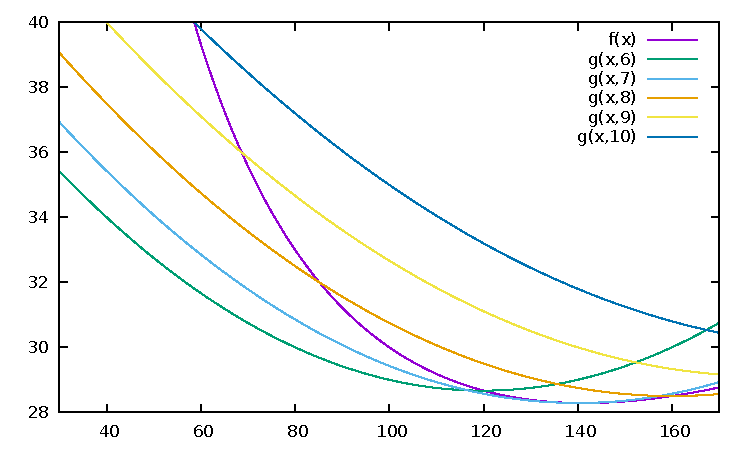
\includegraphics{figures/eoq_loss_0_2}
\end{center}

The situation with $k=0.2$. The $f$ is the graph of the EOQ model, the
$g(x,6)$ is the graph of the cost of the model with loss and with
$T=6$, the $x$ corresponds to the order size $Q$; likewise $g(x,7)$ is
the cost for $T=7$ and so on. We now clearly see that none of the
models with loss achieves a lower cost than the EOQ model with optimal order quantity. 

\begin{center}
  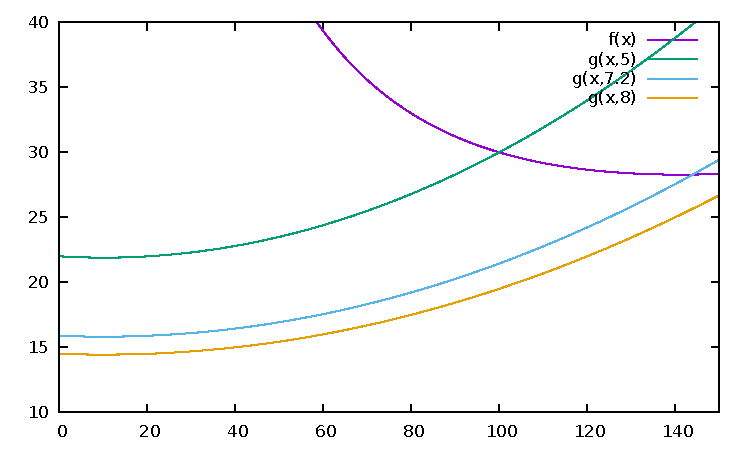
\includegraphics{figures/eoq_loss_0_1}
\end{center}

The situation with $k=0.1$. We now see that when rejecting demand is
pretty cheap, it is best not to order anything: when $Q=0$ the cost is
minimal, hence rejecting all demand seems to be optimal. This is
definitely unexpected!

So, why is that? From the above there seem to be two alternatives,
either order the EOQ and don't reject any demand, or order nothing and
reject all demand.  So, let's trace back the entire analysis.  Indeed,
if we decide to order items and keep them in inventory to satify
demand, then the cost of this must be smaller than the cost of losing
demand. For otherwise, we would simply not be in this business
anyway. So, all in all, this is entirely logical (in hindsight): If
orders are so profitable that you are prepared to keep inventories, it
simply can't be optimal to lose demand. If, however, keeping
inventories is too expensive, it must be optimal not to participate at
all.

Note that this argument is only valid for the case in which everything
is deterministic. In case of stochastic demand, we'll see that
everything changes.

% If we
% reject all demand, then the average cost rate must be $k D$. If, on
% the other hand, we don't want to reject all demand, we order an amount
% $Q$. The cost of ordering is:
% \begin{equation*}
%   \frac A T + \frac{hQ^2}{2DT} - \frac{k Q}{T}.
% \end{equation*}
% Therefore, when this is negative, the overall cost must
% decrease. Thus, if
% \begin{equation*}
%   \frac A T + \frac{hQ^2}{2DT}  < \frac{k Q}{T},
% \end{equation*}
% we must be better off by ordering some amount $Q$. Now it appears that
% all components in this equation are divided by $T$. Removing this
% leads to
% \begin{equation*}
%   A + \frac{hQ^2}{2D}  < k Q.
% \end{equation*}
% But now we see that the cost benefit of ordering $Q$ is independent of
% $T$!



  \end{solution}
\end{question}


\begin{question}
  Continuing on the above question, it might be that items or ordering
  costs are so high that it is better not to `enter the business' at
  all. Can you find a condition to decide whether to keep inventories
  and satisfy demand or reject all demand and have no inventories?
  \begin{solution}
    The cost rate of dropping all demand is $kD$. The cost rate of keeping inventories is, under the EOQ model,  and using that the optimal order quantity $Q^* = \sqrt{2AD/h}$, 
    \begin{equation*}
      \begin{split}
      f(Q^*)
 &= A \frac{D}{Q^*} + \frac h 2 Q \\
 &= A \frac{D}{\sqrt{2AD/h}} + \frac h 2 \sqrt{\frac{2AD}h} \\
 &= A D \sqrt{\frac{h} {2AD}} + \frac h 2 \sqrt{\frac{2AD}h} \\
 &=  \sqrt{\frac {AhD}{2}} + \sqrt\frac{ADh}2 \\
 &=  2\sqrt{\frac {AhD}{2}} \\
 &=  \sqrt{2AhD}.
      \end{split}
    \end{equation*}
When the cost rate of rejecting demand is lower than the cost rate of keeping inventories, we reject the demand, that is, when
\begin{equation*}
kD < \sqrt{2AhD}.
\end{equation*}
We can simplity this a bit to $k^2D^2 < 2AhD$, from which we get
\begin{equation*}
  k^2 D < 2 A h.
\end{equation*}
Thus, when the demand is really small, or the reject cost $k$ is
small, we reject demand. 
  \end{solution}
\end{question}


\begin{question}
  What if we have quantity discounts? What would you do?  
  \begin{solution}
We would need to analyze various alternatives, one alternative for each `ordering regime', since now the ordering cost depends on  the amount we are going to order.

\paragraph{All-unit discounts}

\begin{center}
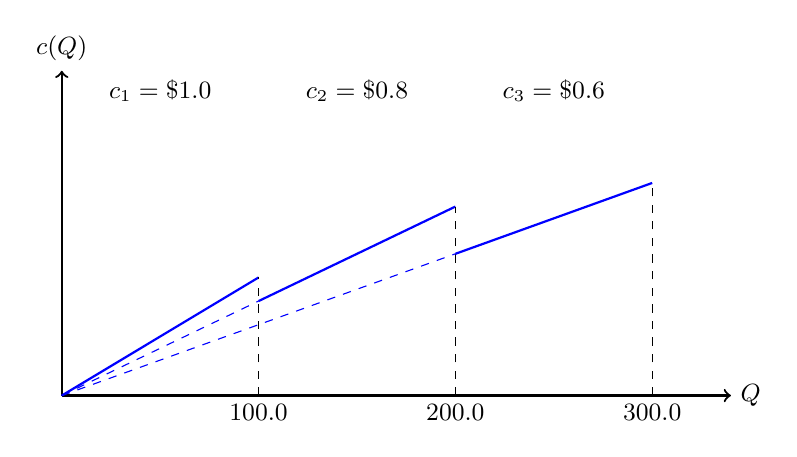
\begin{tikzpicture}[x=0.025cm,y=0.015cm]
\small
\draw[thick,->] (0,0) -- (340,0) node[right] {$Q$};
\draw[thick,->] (0,0) -- (0,275) node[above] {$c(Q)$};
\def\w{100}
\foreach \n/\a in {1/1.0,2/0.8,3/0.6}{
	\pgfmathsetmacro{\s}{(\n-1)*\w}	
	\pgfmathsetmacro{\e}{\n*\w}
	\draw[thick,color=blue,domain=\s:\e] plot (\x,{\a*\x});
	\draw[dashed,color=blue,domain=0:{\s+0.01}] plot (\x,{\a*\x});
	\draw[] (\e,0) -- (\e,0) node[below] {$\e$};
	\draw[dashed] (\e,0) -- (\e,\e*\a);
	\draw[] ({(\s+\e)/2},275) -- ({(\s+\e)/2},275) node[below] {$c_{\n} = \mathdollar\a$};}
\end{tikzpicture}
\end{center}

Average cost per unit time:
\begin{align*}
f(Q) 
& = Kd / Q + cd + hQ/2 \\
& = Kd / Q + cd + \alpha cQ / 2 \quad (h = \alpha c)
\end{align*}

Average cost per unit time:
\begin{equation*}
f(Q) = 
\begin{cases}
Kd / Q + c_1 d + \alpha c_1 Q / 2 & \text{if } 0 \leq Q < Q_1 \\
Kd / Q + c_2 d + \alpha c_2 Q / 2 & \text{if } Q_1 \leq Q < Q_2 \\
Kd / Q + c_3 d + \alpha c_3 Q / 2 & \text{if } Q_2 \leq Q 
\end{cases}
\end{equation*}

\begin{equation*}
f(Q) = 
\begin{cases}
Kd / Q + 1.0 d + \alpha 1.0 Q / 2 & \text{if } 0 \leq Q < 100 \\
Kd / Q + 0.8 d + \alpha 0.8 Q / 2 & \text{if } 100 \leq Q < 200 \\
Kd / Q + 0.6 d + \alpha 0.6 Q / 2 & \text{if } 200 \leq Q 
\end{cases}
\end{equation*}

\begin{equation*}
f(Q) = 
\begin{cases}
2000 / Q + 20 + 0.10 Q & \text{if } 0 \leq Q < 100 \\
2000 / Q + 16 + 0.08 Q & \text{if } 100 \leq Q < 200 \\
2000 / Q + 12 + 0.06 Q & \text{if } 200 \leq Q 
\end{cases}
\end{equation*}

\begin{itemize}
\item $c_1 = \mathdollar 1.0$, $c_2 = \mathdollar 0.8$, $c_3 = \mathdollar 0.6$
\item $Q_1 = 100$, $Q_2 = 200$
\end{itemize}

\begin{itemize}
\item $K = \mathdollar 100$
\item $\alpha = 0.2$, $d = 20$ units
\end{itemize}

\begin{center}
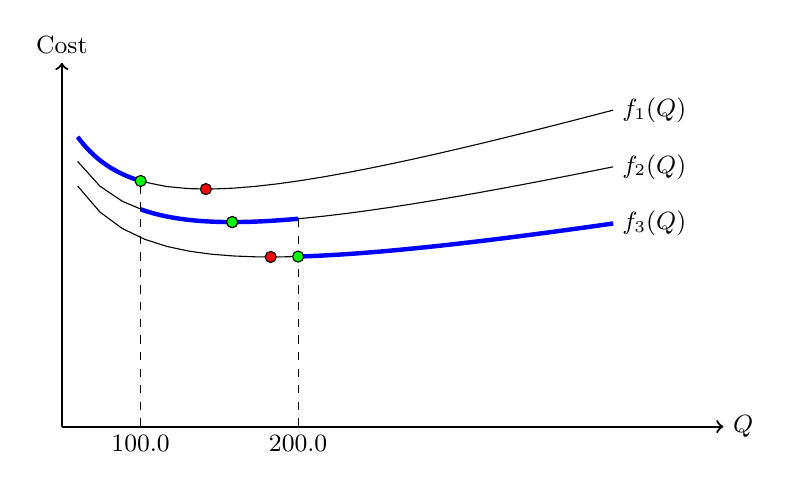
\begin{tikzpicture}[x=0.02cm,y=0.06cm]
\small
\def\c{1} 
\def\K{100} 
\def\h{0.2} 
\def\d{20} 
\def\alpha{0.2}
\def\w{100}
\draw[thick,->] (50,-2) -- (470,-2) node[right] {$Q$};
\draw[thick,->] (50,-2) -- (50,75) node[above] {Cost};
\foreach \n/\c in {1/1.0,2/0.8,3/0.6} {
	\pgfmathsetmacro{\h}{\alpha*\c}	
	\pgfmathsetmacro{\Q}{sqrt(2)*sqrt(\K)*sqrt(\d)/sqrt(\h)}
	\pgfmathsetmacro{\f}{sqrt(2)*sqrt(\K)*sqrt(\d)*sqrt(\h)+\c*\d}	
	\pgfmathsetmacro{\s}{(\n-1)*\w}	
	\pgfmathsetmacro{\e}{\n*\w}

	\draw[domain=60:400] plot (\x,{\d*\K/\x+\c*\d+\h*\x/2}) node[right] {$f_{\n}(Q)$};

	\ifnum\n<3
		\draw[color=blue,ultra thick,domain={max(60,\s}:\e] plot (\x,{\d*\K/\x+\c*\d+\h*\x/2});
		\draw[dashed] (\e,-2) -- (\e,{\d*\K/\e+\c*\d+\h*\e/2});
		\draw (\e,-2) node[below] {$\e$};
	\else
		\draw[color=blue,ultra thick,domain={max(60,\s}:400] plot (\x,{\d*\K/\x+\c*\d+\h*\x/2});
	\fi

	\draw [fill=red] (\Q,\f) circle (2pt);

	\pgfmathparse{int(\Q-\s)}
	\ifnum \pgfmathresult < 0
		\draw [fill=green] (\s,{\d*\K/\s+\c*\d+\h*\s/2}) circle (2pt);
	\fi
	\pgfmathparse{int(\Q-\e)}
	\ifnum \pgfmathresult > 0
		\draw [fill=green] (\e,{\d*\K/\e+\c*\d+\h*\e/2}) circle (2pt);
	\fi
	\pgfmathparse{int((\Q-\e)*(\Q-\s))}
	\ifnum \pgfmathresult < 0
		\draw [fill=green] (\Q,\f) circle (2pt);
	\fi
}
\end{tikzpicture}
\end{center}

Optimization:
\begin{itemize}
\item global optimum $\rightarrow$ check breakpoints and local minimums and compare average total costs
\end{itemize}


\paragraph{incremental discounts}

\begin{center}
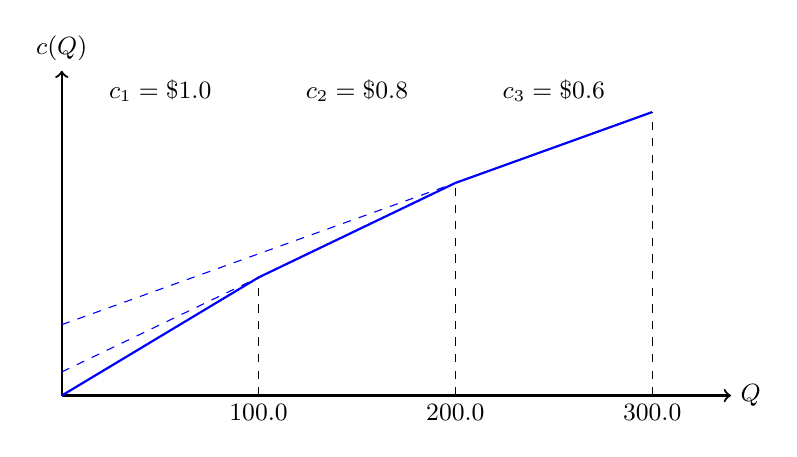
\begin{tikzpicture}[x=0.025cm,y=0.015cm]
\small
\draw[thick,->] (0,0) -- (340,0) node[right] {$Q$};
\draw[thick,->] (0,0) -- (0,275) node[above] {$c(Q)$};
\def\w{100}
\pgfmathsetmacro{\b}{0}
\foreach \n/\a/\b in {1/1.0/0,2/0.8/20,3/0.6/60}{
	\pgfmathsetmacro{\s}{(\n-1)*\w}	
	\pgfmathsetmacro{\e}{\n*\w}
	\draw[thick,color=blue,domain=\s:\e] plot (\x,{\a*\x+\b});
	\draw[dashed,color=blue,domain=0:{\s+0.01}] plot (\x,{\a*\x+\b});
	\draw[] (\e,0) -- (\e,0) node[below] {$\e$};
	\draw[dashed] (\e,0) -- (\e,\e*\a+\b);
	\draw[] ({(\s+\e)/2},275) -- ({(\s+\e)/2},275) node[below] {$c_{\n} = \mathdollar\a$};}
\end{tikzpicture}
\end{center}

Average cost per unit time:
\begin{align*}
f(Q) 
& = Kd / Q + cd + hQ / 2 \\
& = Kd / Q + c(Q)d/Q + \alpha c(Q)/2 \quad (c = c(Q)/Q, h = \alpha c)
\end{align*}

Average variable cost:

\begin{equation*}
c(Q) = 
\begin{cases}
c_1 Q & \text{if } 0 \leq Q < Q_1 \\
c_1 Q_1 + c_2(Q - Q_1) & \text{if } Q_1 \leq Q < Q_2 \\
c_1 Q_1 + c_2(Q_2 - Q_1) + c_3(Q - Q_2) & \text{if } Q_2 \leq Q 
\end{cases}
\end{equation*}


\begin{equation*}
c(Q) = 
\begin{cases}
Q & \text{if } 0 \leq Q < 100 \\
20 + 0.8Q & \text{if } 100 \leq Q < 200 \\
60 + 0.6Q & \text{if } 200 \leq Q 
\end{cases}
\end{equation*}

Average cost per unit time:

\begin{equation*}
f(Q) = Kd / Q + c(Q)d / Q + \alpha c(Q) / 2
\end{equation*}

\begin{equation*}
f(Q) = 2000 / Q + c(Q)20 / Q + 0.1 c(Q)
\end{equation*}

\begin{itemize}
\item $c_1 = \mathdollar 1.0$, $c_2 = \mathdollar 0.8$, $c_3 = \mathdollar 0.6$
\item $Q_1 = 100$, $Q_2 = 200$
\end{itemize}

\begin{itemize}
\item $K = \mathdollar 100$
\item $\alpha = 0.2$, $d = 20$ units
\end{itemize}

Average cost per unit time: (convex for each segment)
\begin{equation*}
f(Q) = 
\begin{cases}
2000 / Q + 20 + 0.10Q & \text{if } 0 \leq Q < Q_1 \\
2400 / Q + 18 + 0.08Q & \text{if } Q_1 \leq Q < Q_2 \\
3200 / Q + 18 + 0.06Q & \text{if } Q_2 \leq Q 
\end{cases}
\end{equation*}

\begin{center}
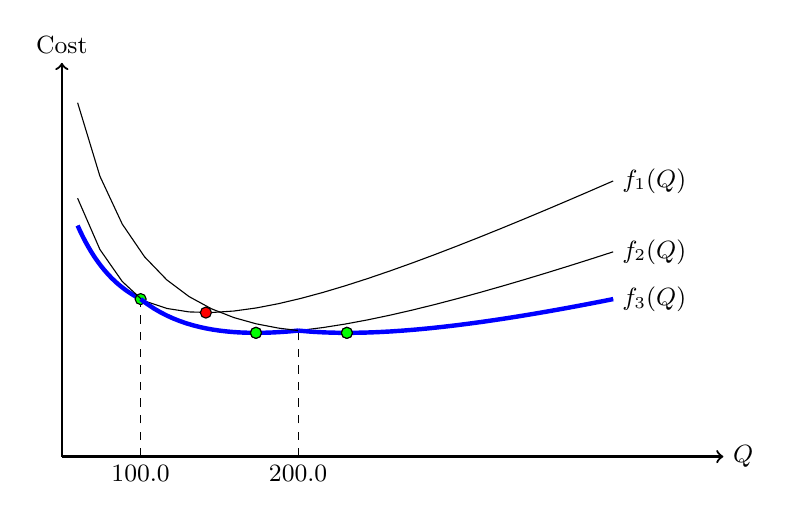
\begin{tikzpicture}[x=0.02cm,y=0.10cm]
\small
\def\c{1} 
\def\K{100} 
\def\h{0.2} 
\def\d{20} 
\def\alpha{0.2}
\def\w{100}
\draw[thick,->] (50,30) -- (470,30) node[right] {$Q$};
\draw[thick,->] (50,30) -- (50,80) node[above] {Cost};
\foreach \n/\a/\b/\c in {1/2000/20/0.1,2/2400/18/0.08,3/3200/18/0.06} {
	\pgfmathsetmacro{\Q}{sqrt(\a)/sqrt(\c)}	
	\pgfmathsetmacro{\f}{\a/\Q+\b+\c*\Q}	
	\pgfmathsetmacro{\s}{(\n-1)*\w}	
	\pgfmathsetmacro{\e}{\n*\w}

	\draw[domain=60:400] plot (\x,{\a/\x+\b+\c*\x}) node[right] {$f_{\n}(Q)$};

	\ifnum\n<3
		\draw[color=blue,ultra thick,domain={max(60,\s}:\e] plot (\x,{\a/\x+\b+\c*\x});
		\draw[dashed] (\e,30) -- (\e,{\a/\e+\b+\c*\e});
		\draw (\e,30) node[below] {$\e$};
	\else
		\draw[color=blue,ultra thick,domain={max(60,\s}:400] plot (\x,{\a/\x+\b+\c*\x});
	\fi

	\draw [fill=red] (\Q,\f) circle (2pt);

	\pgfmathparse{int(\Q-\s)}
	\ifnum \pgfmathresult < 0
		\draw [fill=green] (\s,{\a/\s+\b+\c*\s}) circle (2pt);
	\fi
	\pgfmathparse{int(\Q-\e)}
	\ifnum \pgfmathresult > 0
		\draw [fill=green] (\e,{\a/\e+\b+\c*\e}) circle (2pt);
	\fi
	\pgfmathparse{int((\Q-\e)*(\Q-\s))}
	\ifnum \pgfmathresult < 0
		\draw [fill=green] (\Q,\f) circle (2pt);
	\fi
}
\end{tikzpicture}
\end{center}

Optimization:
\begin{itemize}
\item global optimum $\rightarrow$ check breakpoints and local minimums and compare average total costs
\end{itemize}
  \end{solution}
\end{question}



\begin{question}
EOQ with joint ordering
  \begin{solution}
    TBD
  \end{solution}
\end{question}

\begin{question}
  Consider the setting of the EOQ model but now with batchsize
  constraints, that is, the order quantity is in multiples of some number $q$, say. Can you make a formula for the cost, and find the minimum?
  \begin{solution}
This is, in fact, really easy. Suppose we order $n$ times the minimal order quantity $q$. Then, for a yearly demand $D$, ordering cost $A$, and inventory cost $h$, we pay per year
\begin{equation*}
  A \frac{D}{nq} + h\frac{nq}2 = A\frac{D/q}n + hq\frac{n}2.
\end{equation*}
But this is precisely the normal EOQ model with demand $D'=D/q$ and inventory cost $h'=hq$. Thus, the optimal number of batches to order is:
\begin{equation*}
  n^2 = \frac{2D'A}{h'} = \frac{2AD/q}{hq} = \frac{2AD}{hq^2}.
\end{equation*}
Hence, the optimal $n$ expressed in the EOQ quantity $Q^*$ is 
\begin{equation*}
  n = \sqrt{\frac{2AD}{h}}\frac1q=\frac{Q^*}q.
\end{equation*}
  \end{solution}
\end{question}


\begin{question}
EOQ with yield loss
  \begin{solution}
    TBD
  \end{solution}
\end{question}

\begin{question}
EOQ with lower salvage value
  \begin{solution}
    TBD
  \end{solution}
\end{question}


\begin{question}
EOQ with constraints on cycle length

EOQ under periodic review rather than continuous review.

Constraints on when to order, order moment.

  \begin{solution}
    TBD
  \end{solution}
\end{question}


\begin{question}
  EOQ with positive replenishment lead time and variance in the lead
  time.

  \begin{solution}
    TBD

Suddenly we have to deal with safety stock!
  \end{solution}
\end{question}

\begin{question}
  Suppose that the delivery rate of the items we order is not
  `infinite', as it is in the EOQ setting (recall, in the EOQ we
  assume instantaneous deliveries). If we have a machine that
  replenishes the FGI we have to take into account the production
  rate, $r$ say. If it costs $K$ to switch on the machine, when do you switch the machine on or off?
  \begin{solution}
    An easy policy is to switch the machine on when the FGI level hits
    some level $Q$, and switch it off when the level is $0$. Of course
    we need to assume that $D<r$, i.e., the production rate is larger
    than the demand rate $D$. 

    To find an expression to cover this situation we can reason like
    this.  When the machine is on, inventory increases at rate
    $r-D$. If we keep it on for $T$ time units, then the inventory
    level is $T(r-D)$ when we switch off. The time until the inventory
    hits 0 is then $T(r-D)/D$, since we start with an inventory level
    $T(r-D)$ after switching off and the demand rate is $D$. Thus, the total cycle length is
    \begin{equation*}
      T + \frac{T(r-D)}D = T + T(\frac{r}D-1) = T + T\frac r D - T = T\frac r D.
    \end{equation*}

    What is, in the EOQ, the average inventory cost? It is half the
    maximal height times $h$, i.e., $hQ/2$. In our present case, the
    maximal height is $T(r-D)$. Thus the average inventory cost must
    be  $hT(r-D)/2$. 

    The ordering cost in the EOQ is $A$ times the order frequency, i.e., $A D/Q$. Here the time between two `order' moments (switching moments) is $Tr/D$. Hence, the frequency is $D/rT$ and the average switching cost is $K D/rT$. 

All in all we get for the average cost
\begin{equation*}
  \frac{h(r-D)}2 T + \frac{K}r \frac DT.
\end{equation*}
This is similar to the EOQ model with $h'=h(r-D)$ and $A=K/r$. But then the optimal $T$ must be given by
\begin{equation*}
  T = \sqrt{\frac{2AD}{h'}} = \sqrt{\frac{2DK/r}{h(r-D)}}=\sqrt{\frac{2DK}{hr(r-D)}}.
\end{equation*}
  \end{solution}
\end{question}


\begin{question}
EOQ with variable demand.
  \begin{solution}
    TBD
  \end{solution}
\end{question}

\begin{question}
Wagner Whitin
  \begin{solution}
    TBD
  \end{solution}
\end{question}

\begin{question}
Silver meal
  \begin{solution}
    TBD
  \end{solution}
\end{question}

\begin{question}
Where to put the I/O interface? For what product/item?
  \begin{solution}
    TBD
  \end{solution}
\end{question}

\begin{question}
  What is the difference between continuous and period review? Why/when to prefer one over the other?
  \begin{solution}
    TBD
  \end{solution}
\end{question}

\begin{question}
  What is the difference between fixed order and order-up-to policies?
  Why/when to prefer one over the other?
  \begin{solution}
    TBD

Order quantities

  \end{solution}
\end{question}

\begin{question}
  What  different type of service level can you define?
  Why/when to prefer one over the other?
  \begin{solution}
    TBD

e.g. cycle service level.
  \end{solution}
\end{question}

\begin{question}
  Why to use safefy stock? What is it? 
  \begin{solution}
    TBD
  \end{solution}
\end{question}

\begin{question}
  Are lead times typically (approximately) constant ore variable?
  \begin{solution}
    TBD
  \end{solution}
\end{question}



\subsection{Strategic impact of short leadtimes/small inventories,
  what if lead time is a control?}

You run a pharmaceutical company. The medicines you sell need to be
packaged. The price quotation of the company that prints the packages
depends on the order size $Q$.
  \begin{itemize}
  \item If $Q$ covers 2 weeks of demand: price per unit is 1.15 Euro
  \item If $Q$ covers 1 month of demand: price per unit is 1. Euro
  \item If $Q$ covers 2 months of demand: price per unit is 0.95 Euro
  \item If $Q$ covers 3 months of demand: price per unit is 0.9 Euro
  \item If $Q$ covers 6 months of demand: price per unit is 0.85 Euro
  \end{itemize}
The problem is to determine how much to order.

\begin{question}
  \begin{itemize}
  \item Include your own storage cost, i.e., packages need to be
    stored as your raw materials inventory.  Suppose the
    inventory cost is $20\%$ per unit per year. Can we now compute the
    inventory cost?  Assume that $D = 12000$ units per year.
  \item Include transportation cost.  Assume that $A = 50$ Euro.
  \end{itemize}
\end{question}

\begin{question}
Every so often government regulations change. As a result, the entire
stock becomes obsolete. What now?
\begin{solution}
  \begin{itemize}
  \item Use data to make assumptions on the probability that the
    remaining stock will be affected by a regulation change.
  \item Assume that a regulation change occurs, on average, every
    month, and time to implement the change is one month.
  \item If  $Q$ is 2 weeks of demand, then?  there is no problem
  \item If $Q$ is 3 months of demand, then? 
  \end{itemize}
Challenge: Can you compute the optimal order quantity in this situation? 

%   \begin{lstlisting}%{python}
% A = 50.
% D = 12000
% h = 0.2

% def C(Q, p): # return average yearly inventory cost
%     # p is price per unit, so that
%     # p*h is the inventory cost per unit per year
%     cost = A*D/Q + h*p*Q/2.
%     return cost

% def output(Q, p, period):
%     print("Yearly inventory costs %s: %3.2f; price of a batch: %3.2f"%(period, C(Q, p), Q*p))

% output(D/24, 1.15, "2 weeks")
% #Likewise for the other cases.
%   \end{lstlisting}

%   \begin{minted}{python}
% Yearly costs 2 weeks: 1257.50; batch price: 575.00
% Yearly costs 1 month: 700.00; batch price: 1000.00
% Yearly costs 2 months: 490.00; batch price: 1900.00
% Yearly costs 3 months: 470.00; batch price: 2700.00
% Yearly costs 6 months: 610.00; batch price: 5100.00
%   \end{minted}

What are the consequences?

  \begin{itemize}
    \item For some customers short lead times are very important. So important
      they are willing to pay significantly more per unit.
    \item For some customers small batch sizes are very important. So
      important they are willing to pay significantly more per unit.
    \item Thus,  it is essential for some/many companies to be
      able to offer short and predictable lead times and produce in
      small batches.
    \item Producing in small batches can be achieved with slack capacity and short setup times and low setup costs.
    \item Short and predictable lead times can be achieved with conwip
      and a order prioritization (priority queues)
  \end{itemize}
\end{solution}
\end{question}
